\documentclass[paper=a4, fontsize=11pt]{scrartcl} % A4 paper and 11pt font size

\usepackage[T1]{fontenc} % Use 8-bit encoding that has 256 glyphs
\usepackage[english]{babel} % English language/hyphenation
\usepackage{amsmath,amsfonts,amsthm} % Math packages
\usepackage{graphicx}

\usepackage{lipsum} % Used for inserting dummy 'Lorem ipsum' text into the template

\usepackage{sectsty} % Allows customizing section commands
\allsectionsfont{\centering \normalfont\scshape} % Make all sections centered, the default font and small caps

\usepackage{fancyhdr} % Custom headers and footers
\pagestyle{fancyplain} % Makes all pages in the document conform to the custom headers and footers
\fancyhead{} % No page header - if you want one, create it in the same way as the footers below
\fancyfoot[L]{} % Empty left footer
\fancyfoot[C]{} % Empty center footer
\fancyfoot[R]{\thepage} % Page numbering for right footer
\renewcommand{\headrulewidth}{0pt} % Remove header underlines
\renewcommand{\footrulewidth}{0pt} % Remove footer underlines
\setlength{\headheight}{13.6pt} % Customize the height of the header

\numberwithin{equation}{section} % Number equations within sections (i.e. 1.1, 1.2, 2.1, 2.2 instead of 1, 2, 3, 4)
\numberwithin{figure}{section} % Number figures within sections (i.e. 1.1, 1.2, 2.1, 2.2 instead of 1, 2, 3, 4)
\numberwithin{table}{section} % Number tables within sections (i.e. 1.1, 1.2, 2.1, 2.2 instead of 1, 2, 3, 4)

\setlength\parindent{0pt} % Removes all indentation from paragraphs - comment this line for an assignment with lots of text

%----------------------------------------------------------------------------------------
%	TITLE SECTION
%----------------------------------------------------------------------------------------

\newcommand{\horrule}[1]{\rule{\linewidth}{#1}} % Create horizontal rule command with 1 argument of height

\title{	
	\normalfont \normalsize 
	\textsc{EC500 - Introduction to Learning From Data} \\ [25pt] % Your university, school and/or department name(s)
	\horrule{0.5pt} \\[0.4cm] % Thin top horizontal rule
	\huge Matlab - 2 \\ % The assignment title
	\horrule{2pt} \\[0.5cm] % Thick bottom horizontal rule
}

\author{Mikhail Andreev} % Your name

\date{\normalsize\today} % Today's date or a custom date

\begin{document}
	
	\maketitle % Print the title
	
	%----------------------------------------------------------------------------------------
	%	PROBLEM 1
	%----------------------------------------------------------------------------------------
	
	\section{San Francisco Crime Prediction}
	
	\subsection{Part a}
	
	\hspace*{-4cm}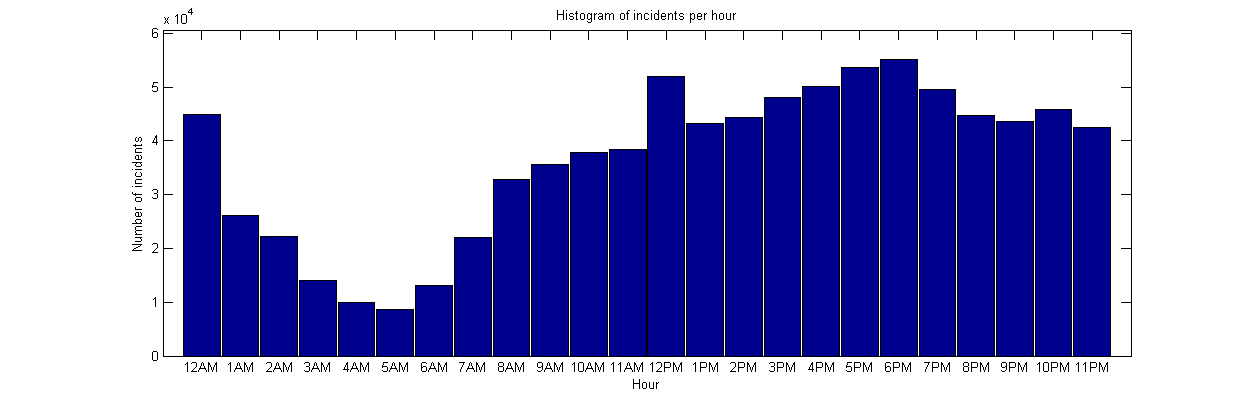
\includegraphics[scale=0.7]{histogram_hours}
	\\\\\\
	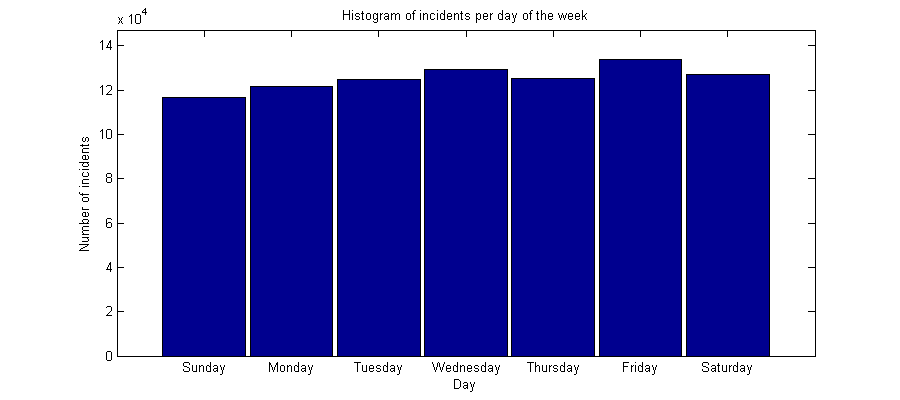
\includegraphics[scale=0.7]{histogram_days}
	\\\\\\
	\hspace*{-3cm}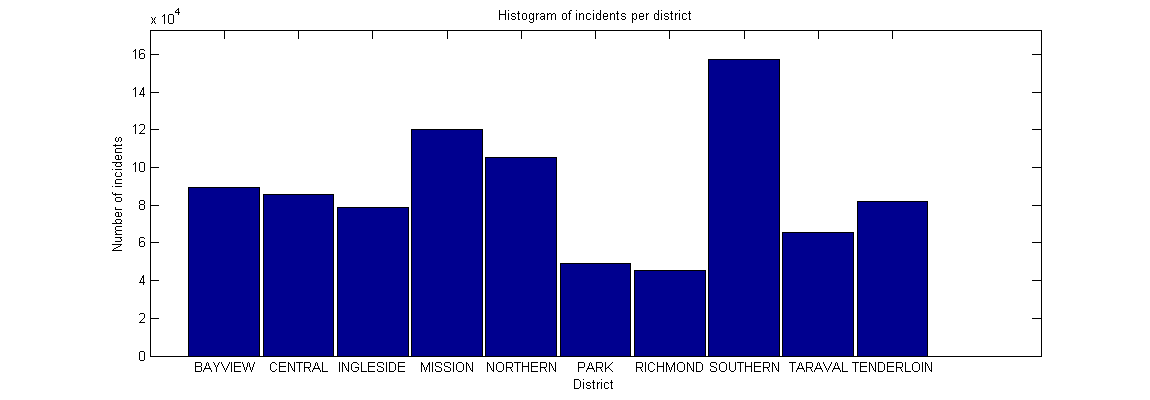
\includegraphics[scale=0.7]{histogram_district}
	\\\\\\
	The list of crimes with the hour they are most likely to occur.\\\\
	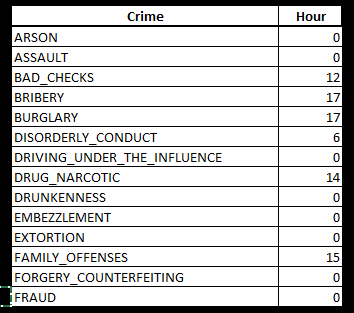
\includegraphics{crimes_hours}
	\\
	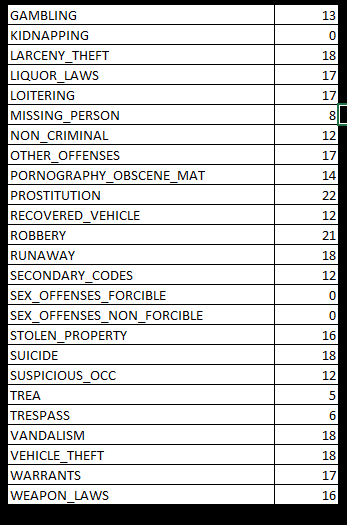
\includegraphics{crimes_hours_2}
	\\\\\\
	The crime most likely to occur in BAYVIEW is OTHER OFFENSES\\
	The crime most likely to occur in CENTRAL is LARCENY and THEFT\\
	The crime most likely to occur in INGLESIDE is OTHER OFFENSES\\
	The crime most likely to occur in MISSION is OTHER OFFENSES\\
	The crime most likely to occur in NORTHERN is LARCENY and THEFT\\
	The crime most likely to occur in PARK is LARCENY and THEFT\\
	The crime most likely to occur in RICHMOND is LARCENY and THEFT\\
	The crime most likely to occur in SOUTHERN is LARCENY and THEFT\\
	The crime most likely to occur in TARAVAL is LARCENY and THEFT\\
	The crime most likely to occur in TENDERLOIN is DRUG and NARCOTIC
	\subsection{Part b}
	
	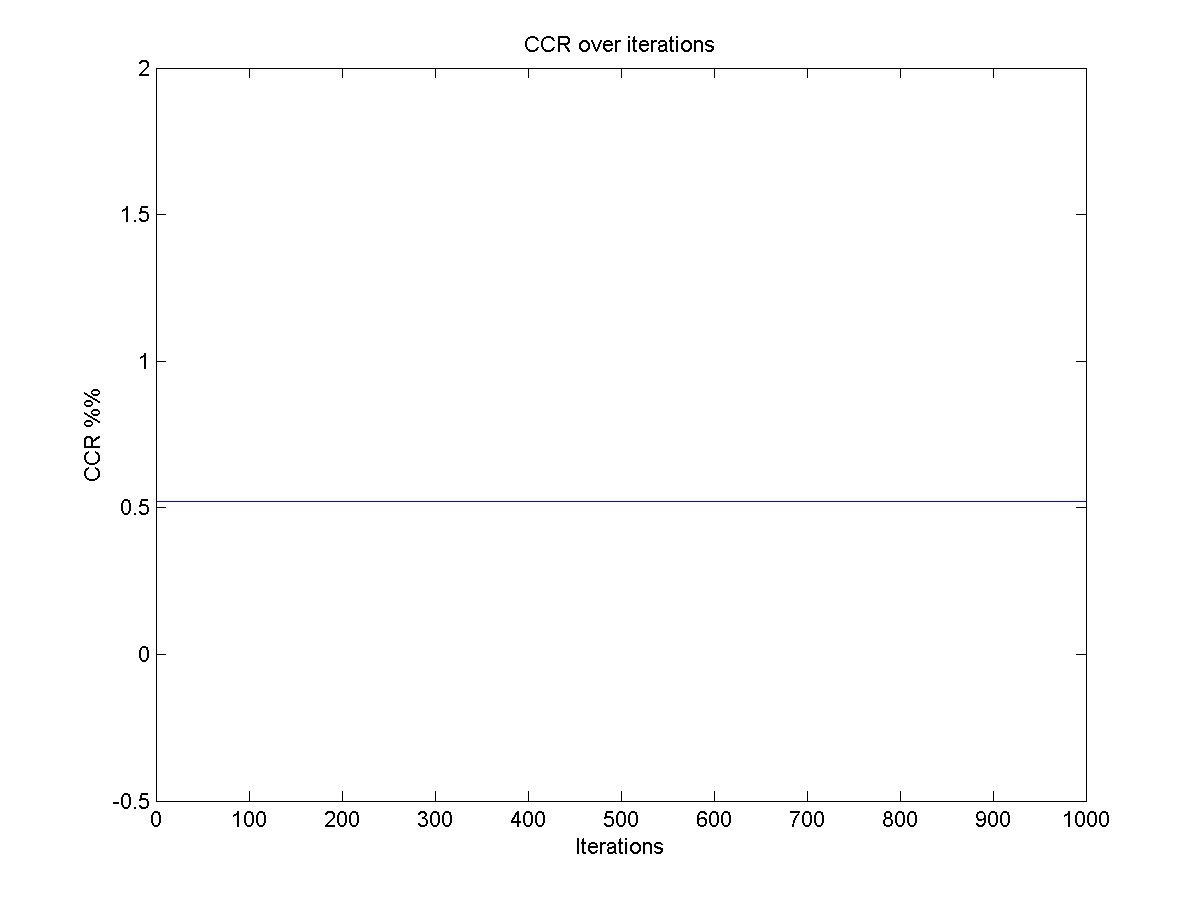
\includegraphics[scale=.8]{CCR}
	\\\\
	This graph indicates that the CCR rate did not noticeably change over the different iterations of the parameters. Unfortunately, this also indicates the CCR rate was very low for the experiment. The end result was only .5\% correct detection.
	\\\\\\
	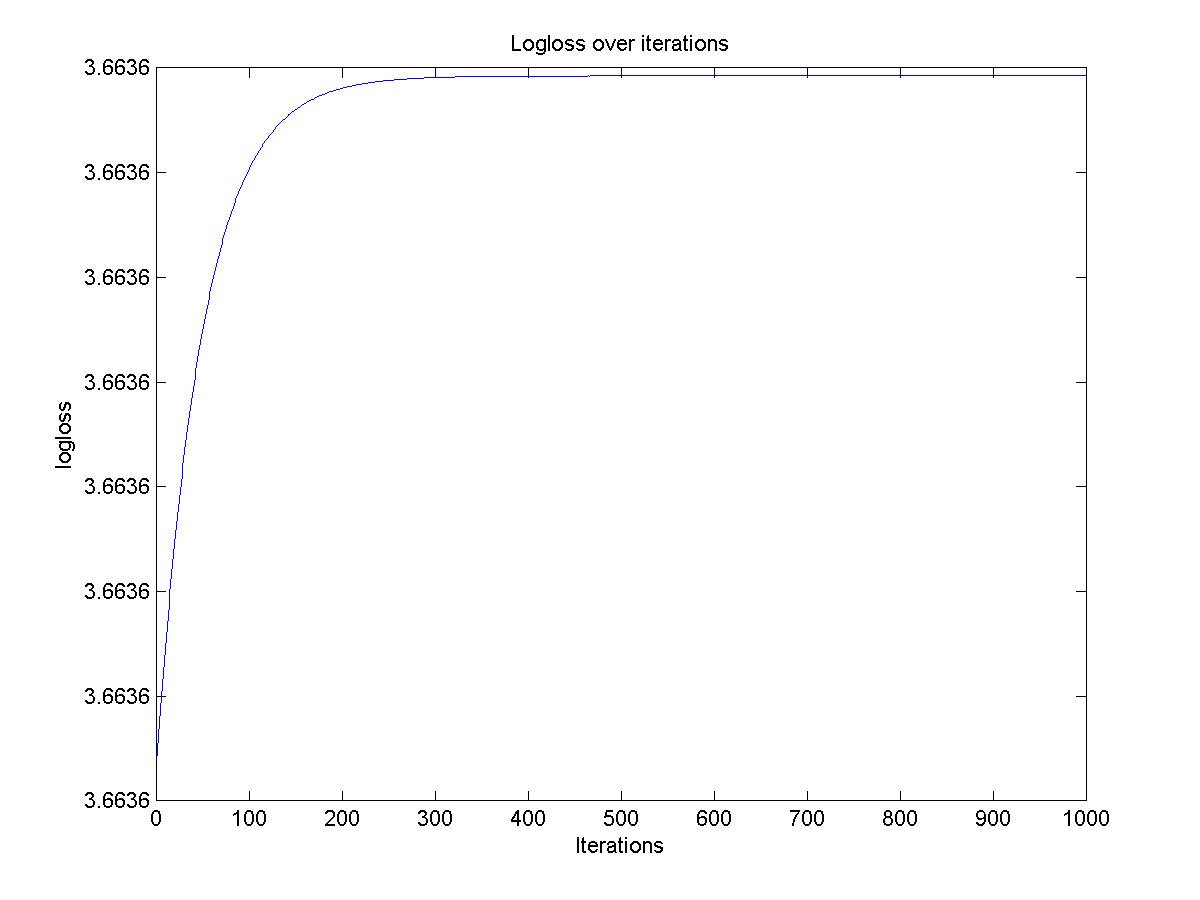
\includegraphics[scale=0.8]{logloss}

	\subsection{Part c}

	
	%----------------------------------------------------------------------------------------
	%	PROBLEM 2
	%----------------------------------------------------------------------------------------
	
	\section{SVM Classifier for Text Documents}
	
	\subsection{Part a}
	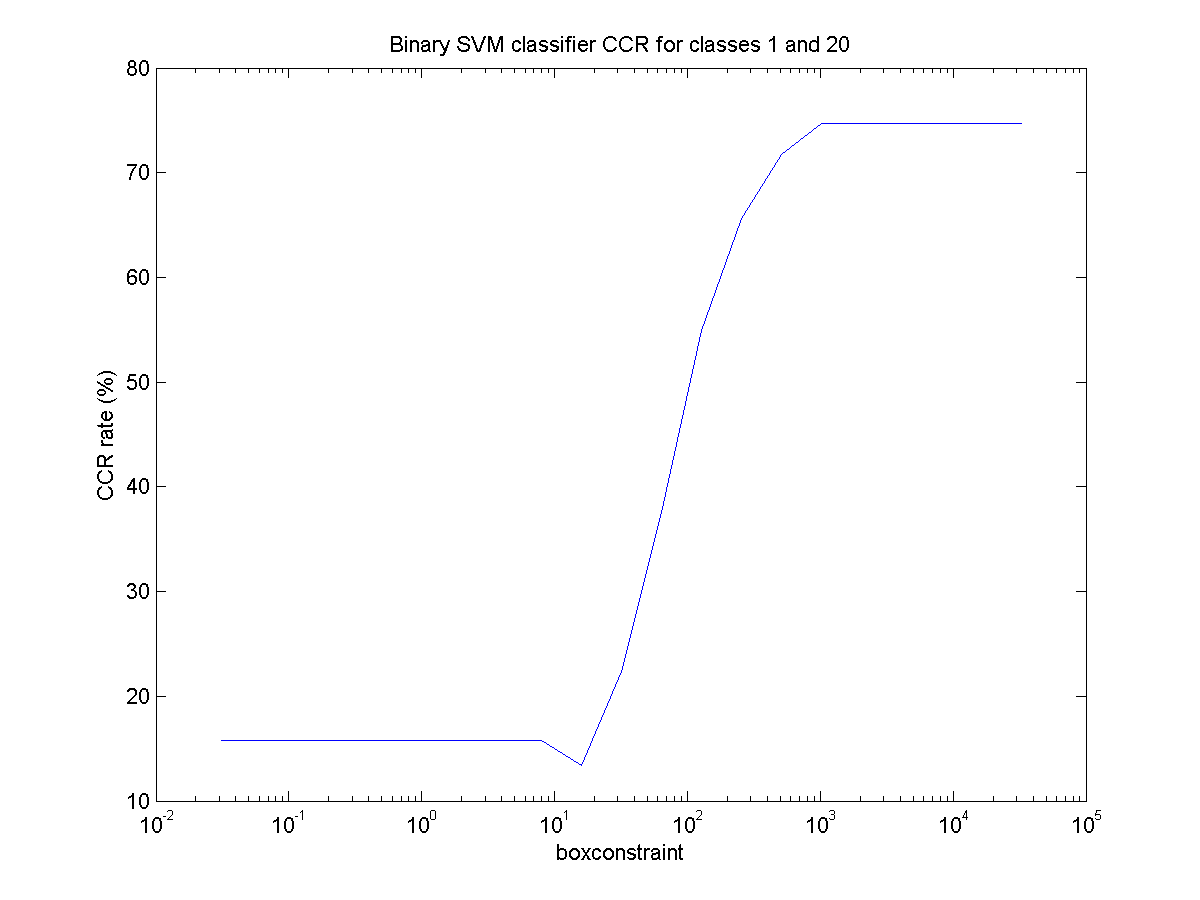
\includegraphics[scale=.8]{part_a_CV_CCR}
	\\\\
	$C^* = 2^{10}$
	\\\\
	$CCR = 80.32\%$

	\subsection{Part b}
	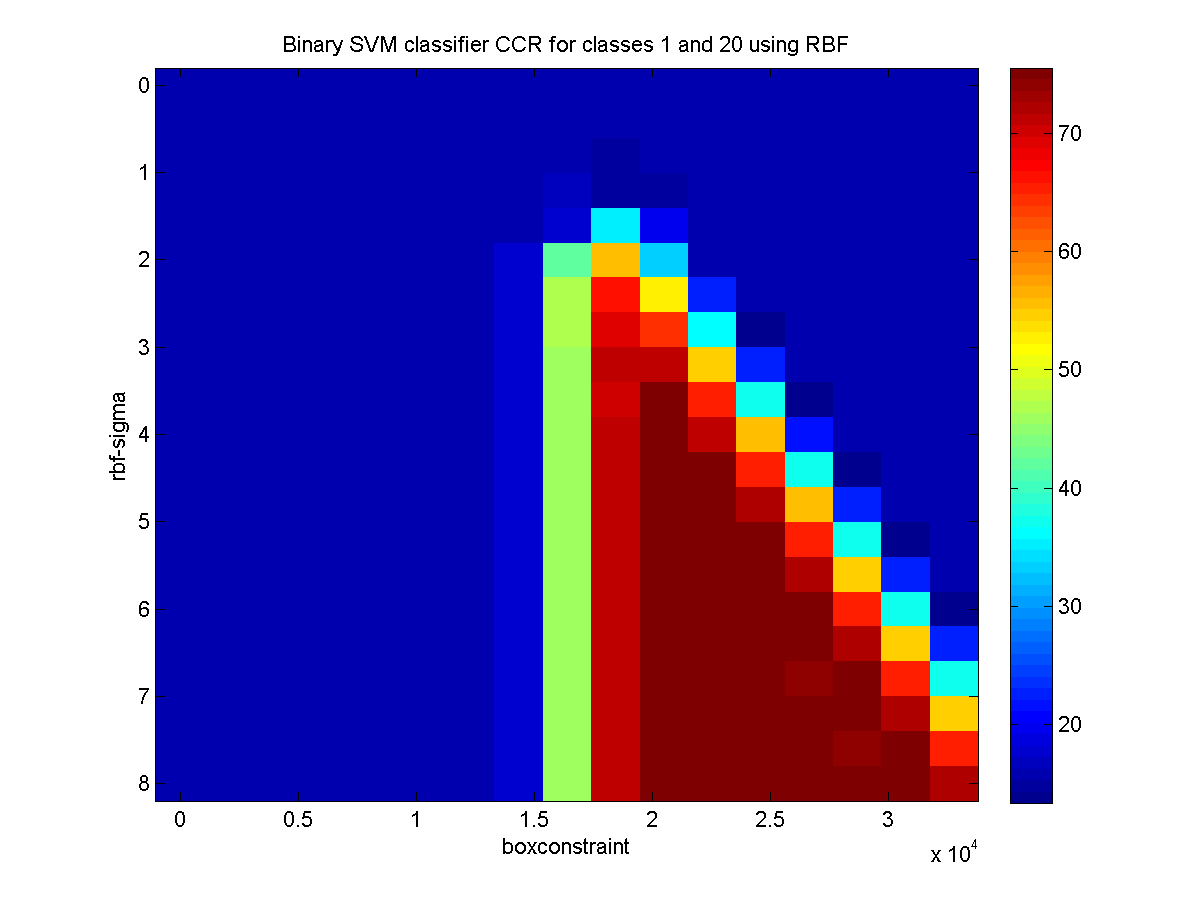
\includegraphics[scale=.8]{part_b_CV_CCR}
	\\\\
	$C^* = 2^{11}$
	\\\\
	$rbf-sigma - 2^{5}$
	\\\\
	$CCR = 79.44\%$
		
	\subsection{Part c}
	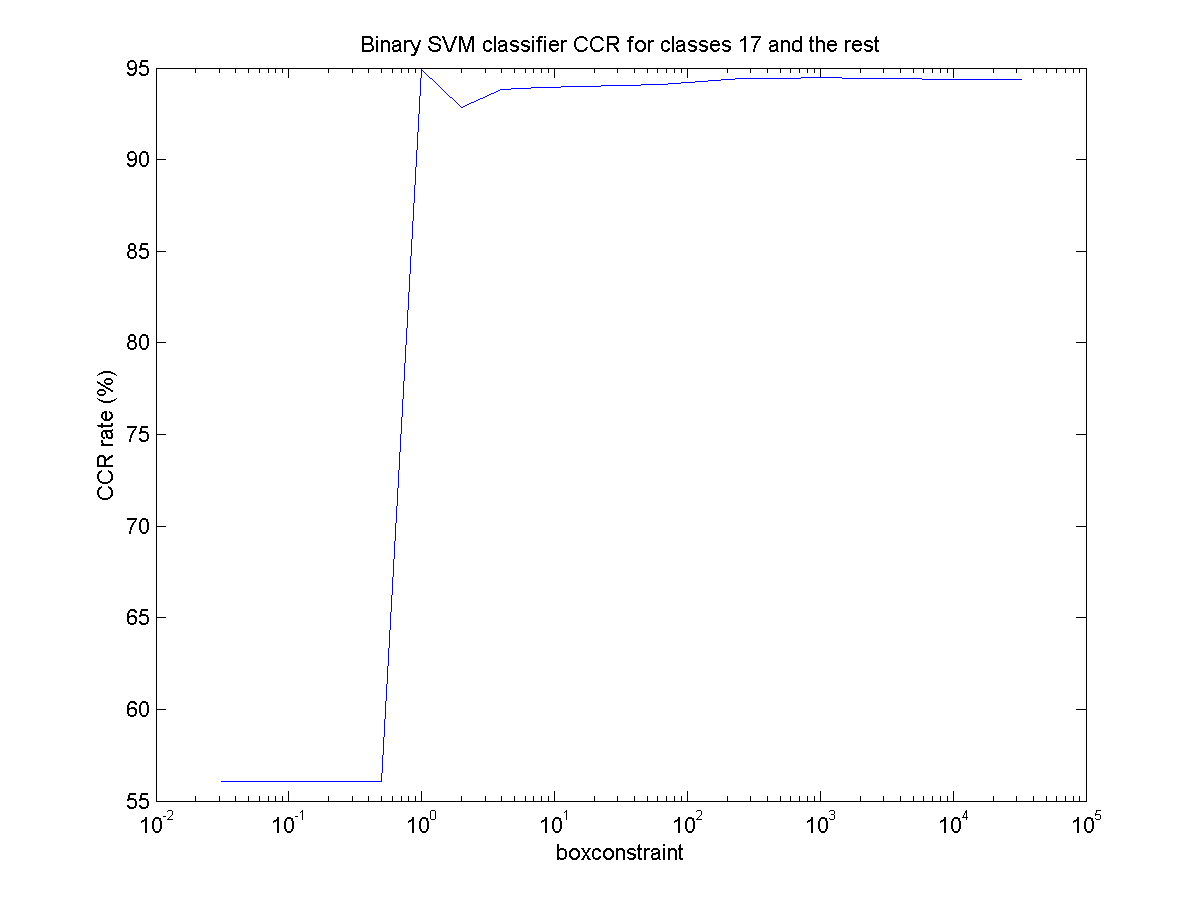
\includegraphics[scale=0.8]{part_c_CV_CCR}
	\\\\
	$C^* = 2^0$
	\\\\
	$CCR = 95.78\%$
	\\\\
	Confusion Matrix:
	\\\\
	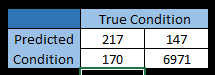
\includegraphics{part_c_confusion_matrix}
	
	\subsection{Part d}
	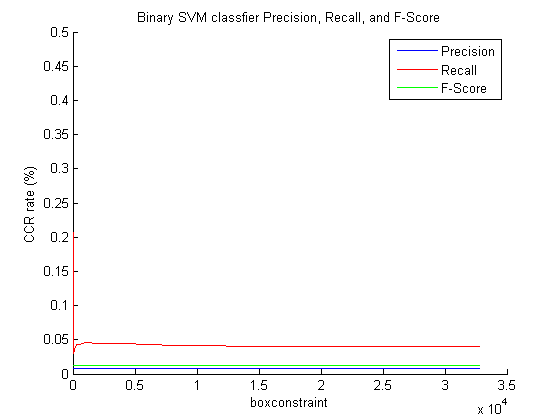
\includegraphics[scale=0.8]{part_d_CV_CCR}
	\\\\
	Best value of C as determined by the precision and the F-score is $2^0$
	\\\\
	Confusion Matrix:
	\\\\
	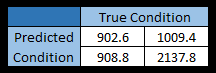
\includegraphics{part_d_confusion_matrix}
	
	
	\subsection{Part e}
	
	\subsection{Part f}
	
\end{document}